\begin{figure}[H]%
	\ThisCenterWallPaper{1}{images/\texorpdfstring{\chaptername\thechapter}}%
	\captionlistentry[figure]{Icon of \chaptername\ \thechapter}% figure with chapter and section number
	%\addcontentsline{lof}{figure}{Icon of \chaptername\ \thechapter}% figure without chapter and section number
	\label{fig:\chaptername\thechapter}%
\end{figure}

\vspace*{-5.15cm}
\epigraph{"Think about \gls{spam} filters; if email didn't come from someone that someone you know knows, that's an important signal, and one we could embed in the environment; we just don't. I just want the world to be filtered through my \gls{social graph}."}{\textit{--- Clay Shirky}}

\noindent\large{\textbf{This {\MakeLowercase{\chaptername}}'s contents:}}
\vspace*{-0.8cm}
\minitoc \mtcskip \minilof
\vspace*{-0.5cm}

In the previous chapter the literature on graph theory concepts, problems, algorithms and on graph database systems was reviewed.
With these concepts fresh in mind it is now possible to go more in depth with graph clustering, community detection in graphs using graph databases.
The chosen GDBMS for storing the data is ArangoDB since it comes with ready to execute algorithms on graphs, has very few feature limitations on its \gls{Community Edition} license and is generally well documented.
The graph dataset that is going to be used contains information of computer science academic publications obtained from \gls{dblp.org}\sfcite{Dagstuhl2021}.
\medskip

The goal of the community detection applied to the \gls{dblp.org}\sfcite{Dagstuhl2021} dataset is to find groups of scientific collaboration between researchers that are more densely connected between them than others.
The dataset contains typical citation data, like authors, title of publications, date, publishers, editors, affiliations etc.
In this chapter, how community detection is carried out - is investigated in the literature. Then, having seen what are the options on the table, will be chosen an algorithm and described the practical part of actually executing it on the graph data.

\section{Literature review of clustering methodologies and algorithms} \label{section:CommunityDetection/Literaturereviewofclusteringmethodologiesandalgorithms}
In this section different graph clustering algorithms are presented.

Some common community detection algorithms are:
\setlist{nolistsep} \begin{itemize}[noitemsep]
	\item \textbf{\gls{Triangle Count}} and \textbf{\gls{Clustering Coefficient}} for overall \gls{relationship density}
	\item \textbf{\gls{Strongly Connected Components} (\acrshort{SCC})} and \textbf{\gls{Weakly Connected Components} (\acrshort{WCC})} for finding connected clusters
	\item \textbf{\gls{Label Propagation}}\sfcite{RaghavanAlbertKumara2007} for quickly inferring groups based on node labels
	\item \textbf{\gls{Louvain Modularity}} for looking at \gls{grouping quality} and \glspl{hierarchy}
	\item \textbf{\gls{InfoMap}} discovers communities by applying the \gls{Random Walk} technique
	\item \textbf{\gls{Leading Eigenvector}} separates the vertices into communities by using the eigenvector of the \gls{modularity matrix} of the graph
	\item \textbf{\gls{Walktrap}} computes the community structure of a network based on a \gls{similarity metric} among vertices
	\item other more specific algorithms\sfcite{Ozturk2014} such as:
        \setlist{nolistsep} \begin{itemize}[noitemsep]
        	\item \textbf{\gls{Hierarchical Clustering}}
        	\item \textbf{\gls{Girvan-Newman Algorithm} (\acrshort{GNA})}
        	\item \textbf{\gls{Algorithm of Duch and Arenas}}
        	\item \textbf{\gls{Algorithm of Clauset} et. al.}
        	\item \textbf{\gls{Newman's Spectral Algorithm}}
        	\item \textbf{\gls{Genetic Algorithm}s} like:
                \setlist{nolistsep} \begin{itemize}[noitemsep]
                	\item \textbf{\gls{Traditional GA}}
                	\item \textbf{\gls{Falkanuer's Grouping Genetic Algorithm}}
                	\item \textbf{\gls{Grouping Genetic Algorithm}} of Tasgin et. al.
                \end{itemize}
        \end{itemize}
\end{itemize}

In \hyperref[longtable:communitydetectionalgorithms]{\autoref{longtable:communitydetectionalgorithms}} are brought descriptions and usecases for some of the algorithms listed above 
- whereas in \hyperref[fig:DaoBothorelLenca2020methodscommunitysizepage27]{\autoref{fig:DaoBothorelLenca2020methodscommunitysizepage27}} is brought a graphical visualization of the distributions of the size of the communities detected with various clustering algorithms.\sfcite{DaoBothorelLenca2020}
After that, the complexity of some of the community detection algorithms is brought in \hyperref[code:PregelPseudocode]{\autoref{code:PregelPseudocode}}. algorithms.\sfcite{LeaoBrandaoVazdeMeloLaender2018, WagensellerIIIWang2017}

\begin{center}
	\vspace*{-0.25cm}
	\begin{longtable}{p{0.22\linewidth}p{0.3475\linewidth}p{0.3475\linewidth}}
		\hline \hline
		\textbf{Algorithm type} & \textbf{What it does} & \textbf{Usecases}\\
		\hline \hline
		\endfirsthead
		
		\multicolumn{3}{l}{... continued from previous page}\\
		\hline \hline
		\textbf{Algorithm type} & \textbf{What it does} & \textbf{Usecases}\\
		\hline \hline
		\endhead
		
		\hline
		\caption*{\tablename\ \thetable{}: \nameref*{longtable:communitydetectionalgorithms}\sfcite{NeedhamHodler2021}. Continues on next page ...}
		\vspace*{0.5cm}
		\endfoot
		
		\hline
		%\multicolumn{2}{| c |}{End of Table}\\
		%\hline
		\caption[Overview of community detection algorithms]{Overview of community detection algorithms\sfcite{NeedhamHodler2021}}
		\label{longtable:communitydetectionalgorithms}
		\vspace*{0.5cm}
		\endlastfoot

		\textbf{Triangle Count and Clu\-s\-ter\-ing Coefficient} & Measures how many nodes form triangles and the degree to which vertices tend to cluster together & Estimating group stability and whether the network might exhibit “small-world” behaviors seen in graphs with tightly knit clusters\\
		\hline
		\textbf{Strongly Con\-nec\-t\-ed Com\-po\-nents} & Finds groups where each vertex is reachable from every other vertex in that same group following the direction of relationships & Making product recommendations based on group affiliation or similar items\\
		\hline
		\textbf{Weakly Connected Com\-po\-nents} & Finds groups where each node is reachable from every other node in that same group, regardless of the direction of relationships & Performing fast grouping for other algorithms and identify islands\\
		\hline
		\textbf{Label Propagation} & Infers clusters by spreading labels based on neighborhood majorities & Understanding consensus in social communities or finding dangerous combinations of possible co-prescribed drugs\\
		\hline
		\textbf{Louvain Modularity} & Maximizes the presumed accuracy of groupings by comparing relationship weights and densities to a defined estimate or average & In fraud analysis, evaluating whether a group has just a few discrete bad behaviors or is acting as a fraud ring\\
		\hline
	\end{longtable}
	\vspace*{-1.35cm}
\end{center}

\begin{figure}[H]%
	\centering%
	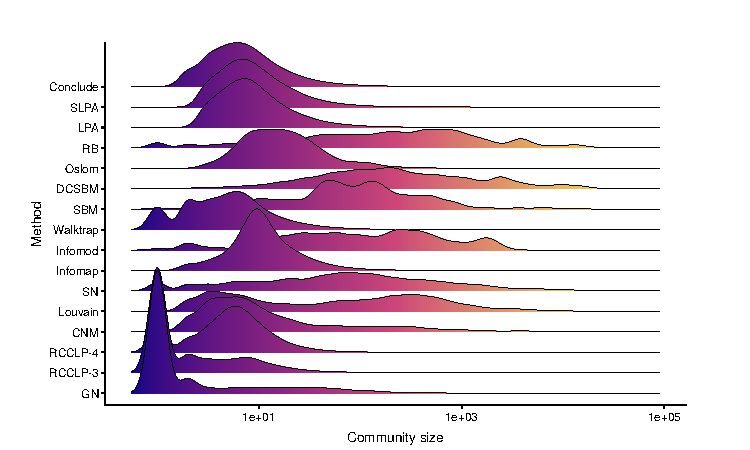
\includegraphics[width=1\textwidth-4pt,%
		bgcolor=white,%
		cfbox=lightestgray % color
			  2pt % rule width
			  0pt % rule separation
			  0pt % margin
	]{images/chapter3/DaoBothorelLenca2020methodscommunitysizepage27.pdf}%
	\caption[Detected community size distributions using different methods, alogrithms]{Detected \gls{community size} distributions using different methods, alogrithms\sfcite{DaoBothorelLenca2020}}%
	\label{fig:DaoBothorelLenca2020methodscommunitysizepage27}%
\end{figure}%

\begin{center}
	\vspace*{-0.25cm}
	\begin{longtable}{p{0.05\linewidth}p{0.383\linewidth}p{0.18\linewidth}p{0.259\linewidth}}
		\hline \hline
		\textbf{Abbr.} & \textbf{Algorithm name} & \textbf{Deterministic or non} & \textbf{Complexity}\\
		\hline \hline
		\endfirsthead
		
		\multicolumn{4}{l}{... continued from previous page}\\
		\hline \hline
		\textbf{Abbr.} & \textbf{Algorithm name} & \textbf{Deterministic or non} & \textbf{Complexity}\\
		\hline \hline
		\endhead
		
		\hline
		\caption*{\tablename\ \thetable{}: \nameref*{longtable:communitydetectionalgorithmscomplexity}. Continues on next page ...}
		\vspace*{0.5cm}
		\endfoot
		
		\hline
		%\multicolumn{2}{| c |}{End of Table}\\
		%\hline
		\caption[Complexity of some of the community detection algorithms]{\gls{Complexity} of some of the community detection algorithms\sfcite{LeaoBrandaoVazdeMeloLaender2018} ($V$, $E$: number of vertices, edges)}
		\label{longtable:communitydetectionalgorithmscomplexity}
		\vspace*{0.5cm}
		\endlastfoot

		\acrshort{LPA} & \gls{Label Propagation} Algorithm & Non-deterministic & $ O \left( V \right) $;\ \ $ O \left( E \right) $\sfcite{WagensellerIIIWang2017}\\
		\hline
		\acrshort{LMA} & \gls{Louvain Modularity} Algorithm & Deterministic & $ O \left( V \log V \right) $\\
		\hline
		\acrshort{IMA} & \gls{InfoMap} Algorithm & Non-deterministic & $ O \left( V \log V \right) $;\ \ $ O \left( E \right) $\sfcite{WagensellerIIIWang2017}\\
		\hline
		\acrshort{GOMA} & \gls{Greedy Optimization} Of Modularity Algorithm & Deterministic & $ O \left( V \log^2\left( V\right) \right) $\\
		\hline
		\acrshort{LEA} & \gls{Leading Eigenvector} Algorithm & Deterministic & $ O \left( V^2 \log V \right) $;\ \ $ O \left( V \left( V + E \right) \right) $\sfcite{WagensellerIIIWang2017}\\
		\hline
		\acrshort{WTA} & \gls{WalkTrap} Algorithm & Non-deterministic & $ O \left( V^2 \log V \right) $\\
		\hline
		\acrshort{EBA} & \gls{Edge Betweenness} Algorithm & Deterministic & $ O \left( V^3 \right) $\\
		\hline
	\end{longtable}
	\vspace*{-1.35cm}
\end{center}

In the following subsections is brought a description of the algorithms and some usage examples.

\subsection[Triangle Count and Clustering Coefficient]{\gls{Triangle Count} and \gls{Clustering Coefficient}} \label{subsection:CommunityDetection/Clusteringmethodologies/TriangleCountandClusteringCoefficient}
\gls{Triangle Count} and \gls{Clustering Coefficient} measures how many nodes form triangles and the degree of community formation between the nodes.\sfcite{NeedhamHodler2021}

\begin{formula}[for the calculation of the clustering coefficient for a node]\label{formula:forthecalculationoftheclusteringcoefficientforanode}\sfcite{NeedhamHodler2021}
	\begin{equation} \stepcounter{equation} \label{equation:forthecalculationoftheclusteringcoefficientforanode}
        CC \left( u \right) = \frac{2R_u}{k_u \left( k_u - 1 \right)}
        \tag{\thechapter.\arabic{equation}}% Use \tag{\thechapter.\arabic{equation}} for chapternumber.equationnumber or \tag{\thesection.\arabic{equation}} for chapternumber.sectionnumber.equationnumber or \tag{\thesubsection.\arabic{equation}} for chapternumber.sectionnumber.subsectionnumber.equationnumber
    \end{equation}
\end{formula}
\medskip

\noindent\textbf{Usecases}

It is principally used to evaluate the stability of groups and if networks show some form of "\gls{small-world}" behavior. Some concrete examples are for classifying \gls{spam} content, community structure of online \gls{social network}s, detection of webpages related to common topics.\sfcite{NeedhamHodler2021}

\noindent where:
\setlist{nolistsep} \begin{itemize}[noitemsep]
	\item $ u $ is a node.
	\item $ R \left( u \right) $ is the number of edges through the neighbors of $ u $.
	\item $ k \left( u \right) $ is the degree of $ u $.
\end{itemize}

\subsection[Strongly Connected Components (SCC) and Weakly Connected Components (WCC)]{\gls{Strongly Connected Components} (\acrshort{SCC}) and \gls{Weakly Connected Components} (\acrshort{WCC})} \label{subsection:CommunityDetection/Clusteringmethodologies/StronglyConnectedComponentsSCCandWeaklyConnectedComponentsWCC}
\gls{Strongly Connected Components} finds groups of vertices where each vertex is reachable from all other other vertices in that same group traversing the edges in their direction. In the case of \gls{Weakly Connected Components} edge direction is irrelevant, so the traversal is done regardless of the direction of the relationships.\sfcite{NeedhamHodler2021}
\medskip

\noindent\textbf{Usecases}

\gls{Strongly Connected Components} and \gls{Weakly Connected Components} are generally used for generation of \gls{recommendation}s, identification of islands or for fast grouping in early steps of \gls{graph analysis}, since they scale nicely. Concrete usecases are the detection of groups of companies whose stakeholders have shares on the other companies of the same group or the analysis of citation networks.\sfcite{NeedhamHodler2021}

\subsection[Label Propagation]{\gls{Label Propagation}} \label{subsection:CommunityDetection/Clusteringmethodologies/LabelPropagation}
\gls{Label Propagation}\sfcite{RaghavanAlbertKumara2007} tries to infer communities by propagating labels on neighbor vertices and detect neighborhood majorities. It is a fast algorithm.\sfcite{NeedhamHodler2021}

The idea behind the algorithm is that in a densely connected community of vertices, a label quickly becomes dominant whereas it is more difficult to do so in a sparsely connected region of the graph.\sfcite{NeedhamHodler2021}

\begin{figure}[H]%
	\centering%
	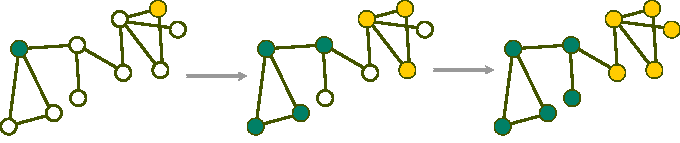
\includegraphics[width=1\textwidth]{images/chapter3/labelpropagation.pdf}%
	\caption[Label propagation algorithm's spread of label to or from neighbors]{Label propagation algorithm's spread of label to or from neighbors}%
	\label{fig:labelpropagation}%
\end{figure}%

There are two ways of propagating the labels, one is the \gls{push method} and the other is the pull. The \gls{pull method} is a better choice when parallelization is involved.
\medskip

\noindent\textbf{The steps of the algorithms}

The pull method of the LPA works as follows:
\setlist{nolistsep} \begin{enumerate}[noitemsep]
	\item Every vertex is labeled with a unique label.
	\item The labels are propagated from vertex to vertex throughout the graph.
	\item At the end of each propagation iteration, each vertex updates its label to match the one with the maximum weight, which is calculated based on the weights of neighbor vertices
and their relationships.
          Ties are broken uniformly and randomly.
	\item Convergence is reached when each vertex is labeled as the majority of its neighbors.
	      It may happen that convergence on a single solution is not reached in a reasonable time.
	      In such cases, a trade-off between accuracy and execution time would be setting a maximum number of iterations to avoid maybe never-ending execution.
\end{enumerate}
This way consensus is reached in groups of vertices.
\medskip

\noindent\textbf{Note}

Should be noted that the algorithm may produce for the same graph different community structures each time it is run.
This happens because the order in which \acrshort{LPA} evaluates the vertices, influences the communities it detects.
A way to reduce the range of possible solutions is by setting preliminary label named "seed labels" to some vertices while others are not labeled.
This way of initialization of the \acrshort{LPA} can be considered a semi-supervised learning to clustering graphs.
\medskip

\noindent\textbf{Usecases}

LPA is mainly used to get an understanding of community consensus in social groups, or for semantic analysis of tweets to classify their polarity as positive or negative.
It finds use also in pharmaceutical fields when dealing with chemical components and their combinations.\sfcite{NeedhamHodler2021}

\subsection[Louvain Modularity]{\gls{Louvain Modularity}} \label{subsection:CommunityDetection/Clusteringmethodologies/LouvainModularity}
\gls{Louvain Modularity} makes use of relationship weights and densities comparisons to maximize the \gls{accuracy of grouping}s.
It is one of the fastest modularity-based algorithms for clustering. Apart from community detection, it reveals also a hierarchy of communities at different scales.\sfcite{NeedhamHodler2021}

\begin{figure}[H]%
	\centering%
	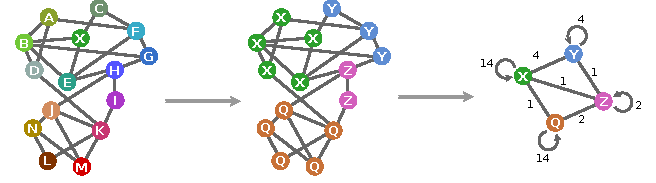
\includegraphics[width=1\textwidth]{images/chapter3/louvainmodularity.pdf}%
	\caption[Louvain Modularity algorithm moving of nodes into higher relationship density groups and aggregating]{Louvain Modularity algorithm moving of nodes into higher relationship density groups and aggregating}%
	\label{fig:louvainmodularity}%
\end{figure}%

To quantify how well a vertex is assigned to a cluster, \acrshort{LMA} looks at the density of connections within a community and compares it to an average or random sample.
This measure is called \textit{modularity}.
Modularity algorithms optimize detected clusters locally and globally.\sfcite{NeedhamHodler2021}
\medskip

\noindent\textbf{The steps of the algorithms}

\setlist{nolistsep} \begin{enumerate}[noitemsep]
	\item "\Gls{greedy}" assignment of nodes to communities, with local optimizations of modularity.
	\item Definition of a more fine-grained network structure based on the clusters found in the first step.
	\item Repeat iteratively the first two steps until no reassignments of communities increase the modularity.
\end{enumerate}
\medskip

\begin{formula}[for the modularity of a group in Louvain Modularity Algorithm]\label{formula:forthemodularityofagroupinLouvainModularityAlgorithm}\sfcite{NeedhamHodler2021}
	\begin{equation} \stepcounter{equation} \label{equation:forthemodularityofagroupinLouvainModularityAlgorithm1}
        M = \Sigma_{c = 1}^{n_c} \left[ \frac{L_c}{L} - \left( \frac{k_c}{2L} \right)^2 \right]
        \tag{\thechapter.\arabic{equation}}% Use \tag{\thechapter.\arabic{equation}} for chapternumber.equationnumber or \tag{\thesection.\arabic{equation}} for chapternumber.sectionnumber.equationnumber or \tag{\thesubsection.\arabic{equation}} for chapternumber.sectionnumber.subsectionnumber.equationnumber
    \end{equation}
\end{formula}

\noindent where:
\setlist{nolistsep} \begin{itemize}[noitemsep]
	\item $ L $ is the number of relationships in the entire group.
	\item $ L_c $ is the number of relationships in a partition.
	\item $ k_c $ is the total degree of nodes in a partition.
\end{itemize}

\begin{formula}[for the first optimization step of Louvain Modularity Algorithm]\label{formula:forthefirstoptimizationstepofLouvainModularityAlgorithm}\sfcite{NeedhamHodler2021}
	\begin{equation} \stepcounter{equation} \label{equation:forthefirstoptimizationstepofLouvainModularityAlgorithm1}
        Q = \frac{1}{2m} \Sigma_{u, v} \left[ A_{uv} - \frac{k_u k_v}{2m} \right] \delta \left(c_u, c_v \right)
        \tag{\thechapter.\arabic{equation}}% Use \tag{\thechapter.\arabic{equation}} for chapternumber.equationnumber or \tag{\thesection.\arabic{equation}} for chapternumber.sectionnumber.equationnumber or \tag{\thesubsection.\arabic{equation}} for chapternumber.sectionnumber.subsectionnumber.equationnumber
    \end{equation}
\end{formula}

\noindent where:
\setlist{nolistsep} \begin{itemize}[noitemsep]
	\item $ u $ and $ v $ are vertices.
	\item $ m $ is the total relationship weight across the entire graph 
	\item $ 2m $ is a common normalization value in modularity formulas.
	\item $ A_{uv} - \frac{k_u k_v}{2m} $ is the strength of the relationship between $ u $ and $ v $ compared to what it is expected with a random assignment of those vertices in the network.
        \setlist{nolistsep} \begin{itemize}[noitemsep]
        	\item $ A_{uv} $ is the weight of the relationship between $ u $ and $ v $.
        	\item $ k_u $ is the sum of relationship weights for $ u $.
        	\item $ k_v $ is the sum of relationship weights for $ v $.
        \end{itemize}
    \item $ \delta \left(c_u, c_v \right) $ is the Kronecker delta function which is equal to 1 if $ u $ and $ v $ are assigned to the same community and 0 otherwise.
\end{itemize}
        
\medskip

\noindent\textbf{Usecases}

It is used in fraud detection or evaluation of unusual behaviors. Similar usecase is the detection of cyberattacks. Another area of application is the detection of hierarchical community structures within the brain's functional network.\sfcite{NeedhamHodler2021}

\section{Chosen algorithm} \label{section:CommunityDetection/Chosenalgorithm}
The algorithm chosen for clustering is the \gls{Label Propagation} Community Detection Algorithm. ArangoDB provides a custom implementation of it, so it is directly applicable on the graph data of the database.

In general, ArangoDB offers a variety of graph processing algorithms, implemented with a custom \gls{Pregel}. \gls{Pregel} is a Distributed Iterative \Glsfirst{graph processing} algorithm developed at \gls{Google} by \citeauthor{MalewiczAusternBikDehnertHornLeiserCzajkowski2009} in \citetitle{MalewiczAusternBikDehnertHornLeiserCzajkowski2009} (\citeyear{MalewiczAusternBikDehnertHornLeiserCzajkowski2009}).\sfcite{MalewiczAusternBikDehnertHornLeiserCzajkowski2009}
It is generally used for graph computations that involve local data, with sparse connections between vertices and whose data is not able to fit all in one computing node.
Some example problems include:
\setlist{nolistsep} \begin{itemize}[noitemsep]
	\item \textbf{\gls{Transportation Routes}}: \Glsfirst{shortest path} algorithms
	\item \textbf{Web}: \gls{PageRank}
	\item \textbf{\Glsfirst{social network}s}: Clustering Techniques
	\item \textbf{Citations Relationships}: \gls{Connected Components}
\end{itemize}

A common \gls{Pregel} algorithm's very high level \gls{pseudocode} is reported in \hyperref[code:PregelPseudocode]{\autoref{code:PregelPseudocode}}.

\noindent\begin{minipage}{\linewidth}% Wraps the lstlisting inside a minipage of width \linewidth with no indentation to prevent it from splitting between pages
	\lstinputlisting[%
		%linerange = {1-29}, % choose line numbers to include
		language = PseudoCode,%
		mathescape = true,%
		label = {code:PregelPseudocode},%
		caption = {[A generic Pregel algorithm's pseudocode]A generic \gls{Pregel} algorithm's \gls{pseudocode}\sfcite{ArangoDBCustomPregel2020}}%
	]{code/PregelPseudocode.pseudo}%
\end{minipage}

Basically it involves two supersteps:
\setlist{nolistsep} \begin{itemize}[noitemsep]
	\item \textbf{\Gls{diffusion}}: information is propagated from vertex to neighbors
	\item \textbf{\Gls{fusion}}: information is aggregated from neighbors to a set of entities
\end{itemize}

\gls{Pregel} is inspired by the Bulk Synchronous Parallel model\sfcite{Valiant1990}, is vertex centric, computes a sequence of iterations (supersteps) in a master-worker model that involves communication between nodes.
The communication is organized via the C++ \acrshort{API} with message passing, no guaranteed order of delivery but knowing that messages are delivered exactly once. \gls{Pregel}s synchronization machanism ensures the absense of deadlocks and data races\sfcite{GonzalesSlides2018}.

\begin{figure}[H]%
	\centering%
	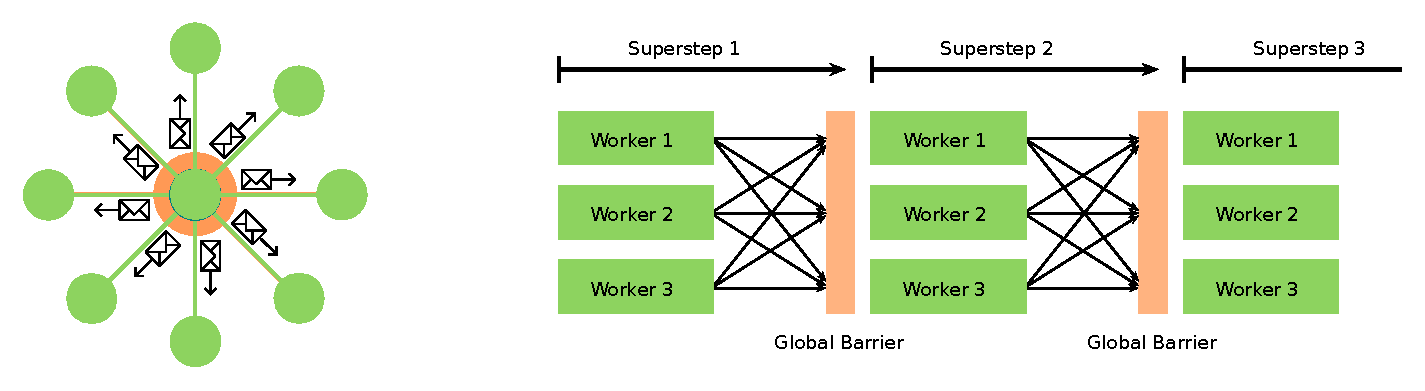
\includegraphics[%
		width=1\textwidth-4pt,%
		bgcolor=white,%
		cfbox=lightestgray % color
			  2pt % rule width
			  0pt % rule separation
			  0pt % margin
	]{images/chapter3/ArangoDBCustomPregel2020sendmessage.pdf}%
	\caption[Pregel's diffusion and fusion computation supersteps]{\gls{Pregel}'s \gls{diffusion} and \gls{fusion} computation supersteps\sfcite{ArangoDBCustomPregel2020}%
	}%
	\label{fig:ArangoDBCustomPregel2020sendmessage}%
\end{figure}%

ArangoDB offers the following custom \gls{Pregel} ready-to-run algorithms:\sfcite{ArangoDBCustomPregel2020, ArangoDBCommunityDetectionPregel2021}
\setlist{nolistsep} \begin{itemize}[noitemsep]
	\item \gls{PageRank}
	\item \gls{Seeded PageRank}
	\item Single-Source \Glsfirst{shortest path}
	\item \gls{Connected Components}
	\setlist{nolistsep} \begin{itemize}[noitemsep]
		\item \gls{Weakly Connected Components} (\acrshort{WCC})
		\item \gls{Strongly Connected Components} (\acrshort{SCC})
	\end{itemize}
	\item \gls{Hyperlink-Induced Topic Search} (HITS)
	\item \gls{Vertex CentralityPermalink}
	\item \gls{Effective Closeness}
	\item \gls{LineRank}
	\item \textbf{Community Detection}
	\setlist{nolistsep} \begin{itemize}[noitemsep]
		\item \textbf{\gls{Label Propagation}}
		\item \gls{Speaker-Listener Label Propagation}
	\end{itemize}
\end{itemize}

As mentioned above, of the two available algorithms for community detection, Label Propagation is chosen to be used.
\bigskip

At initialization, random Community IDs are assigned to the vertices.
Then during each iteration, a vertex sends its current community ID to all its neighbor vertices.
Each vertex adopts the community ID it received most frequently during the iteration.
The algorithm ideally runs until it converges, but this is very unlikely to happen for large graphs.
There is therefore, a need to specify a maximum iteration bound.\sfcite{ArangoDBCommunityDetectionPregel2021}

In the next section are shown all the details of the setup and parameters for the execution of the algorithm.

\section{Clustering collaboration communities - Algorithm execution} \label{section:CommunityDetection/ClusteringcollaborationcommunitiesAlgorithmexecution}
In this section is presented how the clustering is done, with a hands-on approach showing the setup and launch of the algorithm execution and the results afterwards.

\subsection{Execution setup and parameters} \label{subsection:CommunityDetection/ClusteringcollaborationcommunitiesAlgorithmexecution/Executionsetupandparameters}
Before launching the algorithm execution, it is necessary a first step of data preparation in collections of vertices, edges and a graph made out of these.
A brief look at the parameters of the algorithm is given too.

\subsubsection{Environment setup} \label{subsubsection:CommunityDetection/ClusteringcollaborationcommunitiesAlgorithmexecution/Executionsetupandparameters/Environmentsetup}
The setup phase is conducted and described in \hyperref[section:ImplementingtheWebApp/Thedata]{\S\ \ref{section:ImplementingtheWebApp/Thedata} - \nameref{section:ImplementingtheWebApp/Thedata}}, during which the data is prepared, imported, distributed in vertices and edges are defined between them. In the end, a graph is defined using the vertex and edges collections.

Once ready, \texttt{arangosh} is launched from terminal. It is now time to insert the commands with the parameters indicated in the following subsection.

\subsubsection{Parameters used} \label{subsubsection:CommunityDetection/ClusteringcollaborationcommunitiesAlgorithmexecution/Executionsetupandparameters/Parametersused}
Regarding the parameters used in the commands, their values follow:

The parameter regarding the name of the algorithm to use is

\noindent\colorbox{lightestgray}{
	\parbox{1\linewidth-9pt}{%
		\texttt{"labelpropagation"}
	}%
}%

The name of the graph on which to execute the algorithm is:

\noindent\colorbox{lightestgray}{
	\parbox{1\linewidth-9pt}{%
		\texttt{"author\_publisher\_editor\_journal\_publication\_series\_affiliation\_school\_cited\_crossreffed"}
	}%
}%

\noindent The graph contains vertices and edges on authors, publications, affiliation institutions and schools, publishers, editors, journals, cited publications and crossref-fed ones. It also contains data on the year of publication and publication type for the vertices but edges connecting these data are not included in the graph.

The maximum iteration bound chosen is:

\noindent\colorbox{lightestgray}{
	\parbox{1\linewidth-9pt}{%
		\texttt{maxGSS: 100}
	}%
}%

The attribute field of each vertex where to place the result of the computation is:

\noindent\colorbox{lightestgray}{
	\parbox{1\linewidth-9pt}{%
		\texttt{resultField: "community"}%
	}%
}%

\subsection{Algorithm launch} \label{subsection:CommunityDetection/ClusteringcollaborationcommunitiesAlgorithmexecution/Algorithmlaunch}
After having inserted the parameters from the above section, the command is launched.

The execution is fairly straightforward, with just a few lines of code:

First of it is necessary to have shell access to the machine(s) where ArangoDB is installed.
Start by launching \texttt{arangosh} with the shown parameter.

\begin{sublstlisting}%
	\noindent\begin{minipage}{\linewidth}% Wraps the lstlisting inside a minipage of width \linewidth with no indentation to prevent it from splitting between pages
		\lstinputlisting[
			nolol,% will not appear in list of code listings
			linerange = {1-2},% choose line numbers to include
			firstnumber = 1,%
			language = JavaScript,%
			mathescape = true,%
			label = {code:ArangoDBPregelLabelPropagationAlgorithm1},%
			caption = {Launch \texttt{arangosh}}%
		]{code/ArangoDBPregelLabelPropagationAlgorithm.js}%
	\end{minipage}%
	
	Then proceed to setting which database is going to be used.
	It should have all the vertex and edge collections as well as the graph on which the community detection algorithm is going to be run.
	
	\noindent\begin{minipage}{\linewidth}% Wraps the lstlisting inside a minipage of width \linewidth with no indentation to prevent it from splitting between pages
		\lstinputlisting[%
			nolol,% will not appear in list of code listings
			linerange = {3-4},% choose line numbers to include
			firstnumber = 3,%
			language = JavaScript,%
			mathescape = true,%
			label = {code:ArangoDBPregelLabelPropagationAlgorithm3},%
			caption = {Select the database to use}%
		]{code/ArangoDBPregelLabelPropagationAlgorithm.js}%
	\end{minipage}%
	
	After that it is time to import \gls{Pregel} defined algorithms from \texttt{@arangodb}
	
	\noindent\begin{minipage}{\linewidth}% Wraps the lstlisting inside a minipage of width \linewidth with no indentation to prevent it from splitting between pages
		\lstinputlisting[%
			nolol,% will not appear in list of code listings
			linerange = {5-6},% choose line numbers to include
			firstnumber = 5,%
			language = JavaScript,%
			mathescape = true,%
			label = {code:ArangoDBPregelLabelPropagationAlgorithm5},%
			caption = {Import Pregel}%
		]{code/ArangoDBPregelLabelPropagationAlgorithm.js}%
	\end{minipage}%
	
	and go on with the instruction that was discussed in \hyperref[subsubsection:CommunityDetection/ClusteringcollaborationcommunitiesAlgorithmexecution/Executionsetupandparameters/Parametersused]{\S\ \ref{subsubsection:CommunityDetection/ClusteringcollaborationcommunitiesAlgorithmexecution/Executionsetupandparameters/Parametersused} - \nameref{subsubsection:CommunityDetection/ClusteringcollaborationcommunitiesAlgorithmexecution/Executionsetupandparameters/Parametersused}}.
	That will start the execution of the algorithm.

	\noindent\begin{minipage}{\linewidth}% Wraps the lstlisting inside a minipage of width \linewidth with no indentation to prevent it from splitting between pages
    	\noindent\lstinputlisting[%
    		nolol,% will not appear in list of code listings
    		linerange = {7-15},% choose line numbers to include
    		firstnumber = 7,%
    		language = JavaScript,%
    		mathescape = true,%
    			label = {code:ArangoDBPregelLabelPropagationAlgorithm7},%
    			caption = {Start the execution of the algorithm}%
    	]{code/ArangoDBPregelLabelPropagationAlgorithm.js}%
	\end{minipage}%
	
	In order to check the progress of the computation, a status check can be repeatedly obtained with the command in line 17 of \hyperref[code:ArangoDBPregelLabelPropagationAlgorithm16]{\autoref{code:ArangoDBPregelLabelPropagationAlgorithm16}}.
	
	\noindent\begin{minipage}{\linewidth}% Wraps the lstlisting inside a minipage of width \linewidth with no indentation to prevent it from splitting between pages
		\lstinputlisting[%
			nolol,% will not appear in list of code listings
			linerange = {16-17},% choose line numbers to include
			firstnumber = 16,%
			language = JavaScript,%
			mathescape = true,%
			label = {code:ArangoDBPregelLabelPropagationAlgorithm16},%
			caption = {Periodically check for the completion progress}%
		]{code/ArangoDBPregelLabelPropagationAlgorithm.js}%
	\end{minipage}%
\end{sublstlisting}%
\setcounter{lstlisting}{\value{parentlstlisting}-1}%
\vspace*{-5.7pt}%
\begin{lstlisting}[%
	label = {code:ArangoDBPregelLabelPropagationAlgorithm},%
	caption = {[Commands to run to execute the community detection algorithm]Commands to run to execute the community detection algorithm},%
	framesep=0pt,%
	framerule=0pt,%
	frame={tb}%
]
\end{lstlisting}

With the machines involved in this project (see \hyperref[subsection:ImplementingtheWebApp/Thehardware/Themachines]{\S\ \ref{subsection:ImplementingtheWebApp/Thehardware/Themachines} - \nameref{subsection:ImplementingtheWebApp/Thehardware/Themachines}} on \hyperref[subsection:ImplementingtheWebApp/Thehardware/Themachines]{page \pageref*{subsection:ImplementingtheWebApp/Thehardware/Themachines}}) and the chosen number of iterations, it takes about two hours to compute the clusters of collaboration communities.

\subsection{Results} \label{subsection:CommunityDetection/ClusteringcollaborationcommunitiesAlgorithmexecution/Results}
In the end the result of the detected community of a specific vertex is as shown in \hyperref[fig:PregelDetectedCommunityResult]{\autoref{fig:PregelDetectedCommunityResult}}, by means of a new attribute field of named \texttt{community}.

\begin{figure}[H]%
	\centering%
	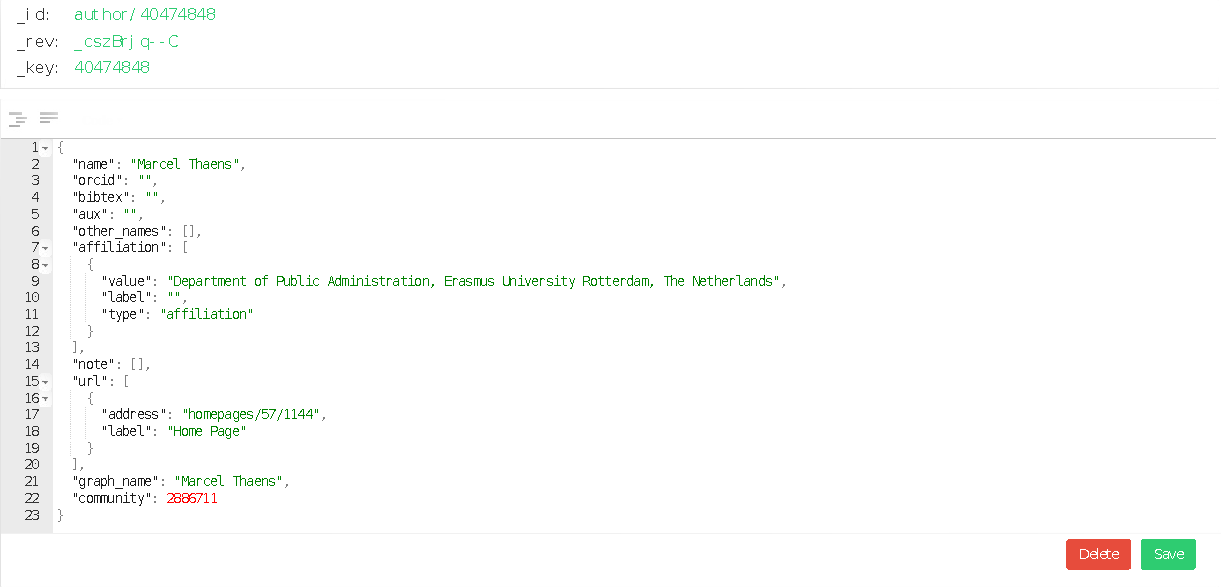
\includegraphics[%
		width=1\textwidth-4pt,%
		bgcolor=white,%
		cfbox=lightestgray % color
			  2pt % rule width
			  0pt % rule separation
			  0pt % margin
	]{images/chapter3/PregelDetectedCommunityResult.pdf}%
	\caption[Collection document representing a vertex of the graph whose membership to a community has been identified]{Collection document representing a vertex of the graph whose membership to a community has been identified}%
	\label{fig:PregelDetectedCommunityResult}%
\end{figure}%

Each detected community has an identifier, a distinct number.
To all the vertices found as members of a community is added the \texttt{community} property and its value is set to the identifier of the belonging community.

In the table below are reported some numbers on the results:
\begin{center}
	\vspace*{-0.25cm}
	\begin{longtable}{p{0.22\linewidth}p{0.3475\linewidth}p{0.3475\linewidth}}
		\hline \hline
		\textbf{Vertex type} & \hfill\textbf{Number of vertices} & \hfill\textbf{Number of detected communities}\\
		\hline \hline
		\endfirsthead
		
		\multicolumn{3}{l}{... continued from previous page}\\
		\hline \hline
		\textbf{Vertex type} & \hfill\textbf{Number of vertices} & \hfill\textbf{Number of detected communities}\\
		\hline \hline
		\endhead
		
		\hline
		\caption*{\tablename\ \thetable{}: \nameref*{longtable:communitydetectionresults}. Continues on next page ...}
		\vspace*{0.5cm}
		\endfoot
		
		\hline
		%\multicolumn{2}{| c |}{End of Table}\\
		%\hline
		\caption[Summary of the community detection results]{Summary of the community detection results}\label{longtable:communitydetectionresults}
		\vspace*{0.5cm}
		\endlastfoot
        
		author & \hfill$ 2786113 $ & \hfill$ 177592 $\\
		\hline
		editor & \hfill$ 43644 $ & \hfill$ 9837 $\\
		\hline
		institution & \hfill$ 56918 $ & \hfill$ 25415 $\\
		\hline
		journal & \hfill$ 1905 $ & \hfill$ 1896 $\\
		\hline
		publication & \hfill$ 5662747 $ & \hfill$ 141939 $\\
		\hline
		publisher & \hfill$ 2292 $ & \hfill$ 1437 $\\
		\hline
		school & \hfill$ 2098 $ & \hfill$ 1677 $\\
		\hline
		series & \hfill$ 1742 $ & \hfill$ 934 $\\
		\hline\hline
		all types & \hfill$ 8557459 $ & \hfill$ 187451 $\\
		\hline
	\end{longtable}
	\vspace*{-1.35cm}
\end{center}

In \hyperref[fig:PregelDetectedCommunityOtherVerticesQuery]{\autoref{fig:PregelDetectedCommunityOtherVerticesQuery}} (the query) and \hyperref[fig:PregelDetectedCommunityOtherVerticesResult]{\autoref{fig:PregelDetectedCommunityOtherVerticesResult}} (the result) are shown in a graph vertices of hop distance 1 to 4 from the start vertex displayed in \hyperref[fig:PregelDetectedCommunityResult]{\autoref{fig:PregelDetectedCommunityResult}}.

\begin{figure}[H]%
	\centering%
	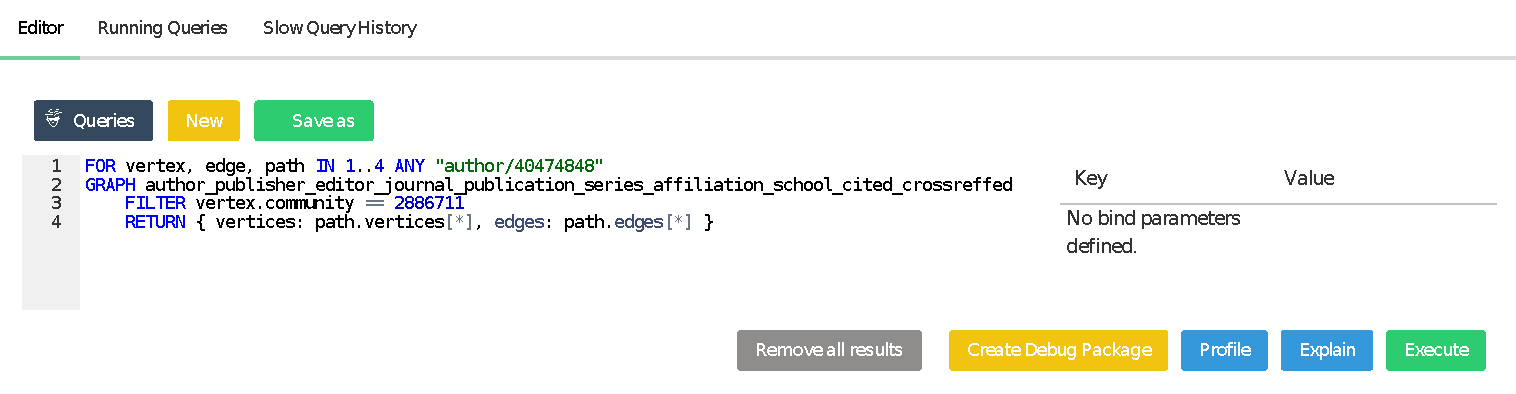
\includegraphics[%
		width=1\textwidth-4pt,%
		bgcolor=white,%
		cfbox=lightestgray % color
			  2pt % rule width
			  0pt % rule separation
			  0pt % margin
	]{images/chapter3/PregelDetectedCommunityOtherVerticesQuery.pdf}%
	\caption[Querying about the neighborhood of a vertex after community detection]{Querying about the neighborhood of a vertex after community detection}%
	\label{fig:PregelDetectedCommunityOtherVerticesQuery}%
\end{figure}%

\begin{figure}[H]%
	\centering%
	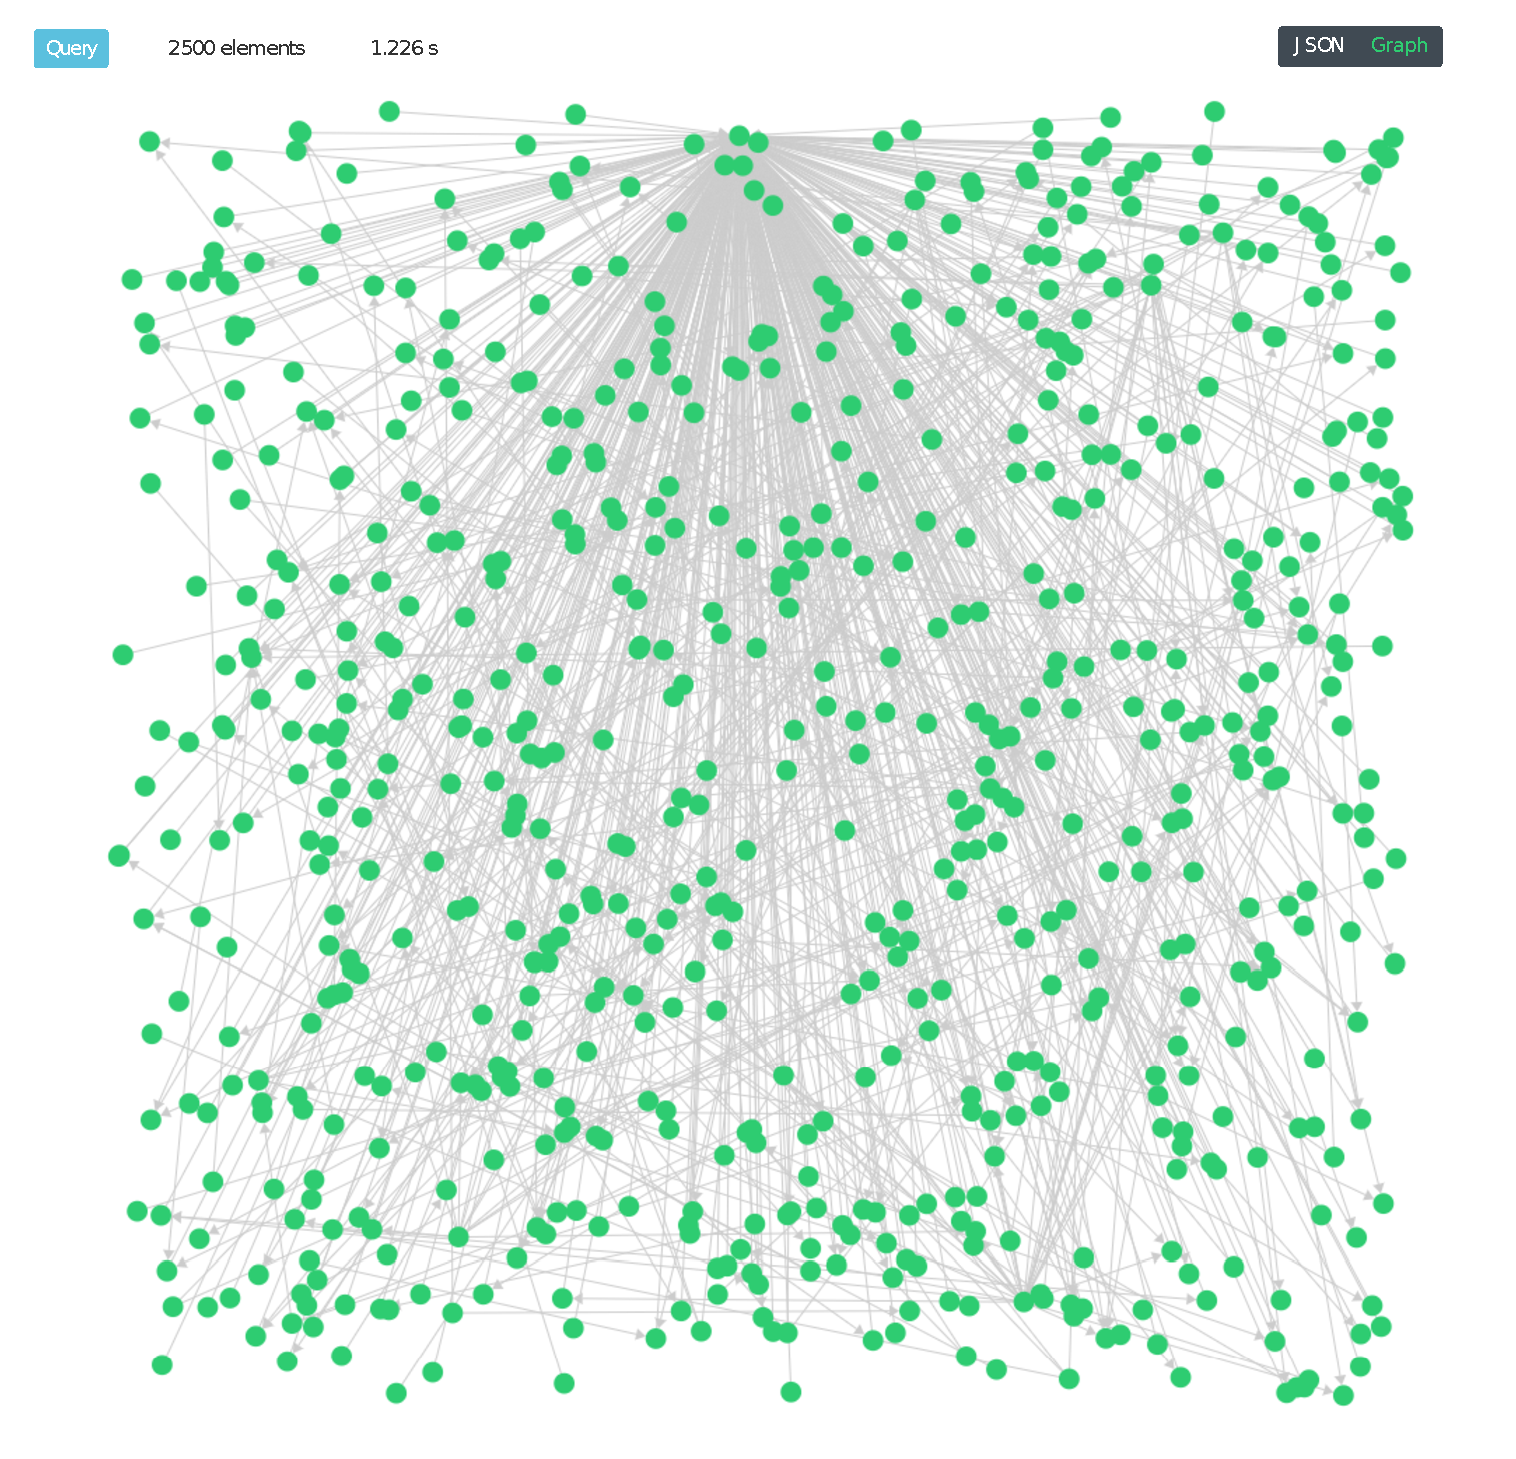
\includegraphics[%
		width=1\textwidth-4pt,%
		bgcolor=white,%
		cfbox=lightestgray % color
			  2pt % rule width
			  0pt % rule separation
			  0pt % margin
	]{images/chapter3/PregelDetectedCommunityOtherVerticesResult.pdf}%
	\caption[Result of the query (in \autoref*{fig:PregelDetectedCommunityOtherVerticesQuery}) on the neighborhood of a vertex after community detection]{Result of the query (in \hyperref[fig:PregelDetectedCommunityOtherVerticesQuery]{\autoref{fig:PregelDetectedCommunityOtherVerticesQuery}}) on the neighborhood of a vertex after community detection}%
	\label{fig:PregelDetectedCommunityOtherVerticesResult}%
\end{figure}%

As can be seen from the graph it is not clear which vertices belong to which communities, even though information on the detected communities is present in the database. Because of these limitations on graphical coloring or grouping the nodes on the ArangoDB web interface, in the next chapter is going to be developed an ad-hoc \gls{Web Application}.
The goal is to display in a graphically understandable manner, groups of nodes and to which community they belong to.

\newpage
\thispagestyle{empty}
